\documentclass[11pt]{article}
\usepackage{tikz}\usetikzlibrary{positioning}
\usepackage[margin=1in]{geometry}
\usepackage{fontspec}
\usepackage{longtable,array}
\usepackage{xcolor}
\definecolor{epgreen}{HTML}{428A5F}
\definecolor{epdarkgreen}{HTML}{214D35}
\usepackage[hidelinks]{hyperref}
\setlength{\parindent}{0pt}
\setlength{\parskip}{5pt}
\emergencystretch=3em
\sloppy
\title{Will September CPI rise more than 0.2\%?}
\author{\href{https://www.expectedparrot.com/}{\textcolor{epgreen}{\textbf{Expected Parrot}}}\\{\small Open-source research tools}\\[4pt]{\small Vorhersage | Forecast research report}}
\date{2026-09-16T22:31:28.278519Z}
\begin{document}
\maketitle
{\color{epgreen}\hrule height 1.5pt}\vspace{8pt}
\section*{\textcolor{epdarkgreen}{Assessment}}
Our sealed estimate is 66.9\%; Kalshi’s opening midpoint was 98.5\%. Current gasoline data changed the model sharply, but a 31.6-point disagreement remains. This non-weather case exposes a concrete process weakness: we adjusted the expected CPI increase without validating the uncertainty of the complete model.


\section*{\textcolor{epdarkgreen}{What counts as Yes?}}
Kalshi contract KXCPI-26SEP-T0.2 concerns the signed, seasonally adjusted monthly increase in the all-items Consumer Price Index for All Urban Consumers (CPI-U) for September 2026. It is not annual inflation or core inflation. The BLS figure must be greater than 0.2\% when published to one decimal place: ordinarily 0.3\% or higher.


The release is scheduled for October 14 at 8:30 a.m. Eastern. The market-specific rules close trading five minutes earlier. Delay, shutdown, no-data fallback and review provisions are retained in the contract record. Our numerical model assumes an ordinary release; it does not separately model those exceptional cases.


\clearpage
\section*{\textcolor{epdarkgreen}{Methodology at a glance}}
The market quote stayed in a separate evaluator store until the forecast was sealed. The reference window, formula and gasoline adjustment were specified before data extraction. Blue boxes contain evidence, amber boxes assumptions, and green boxes calculated results.


\begin{center}
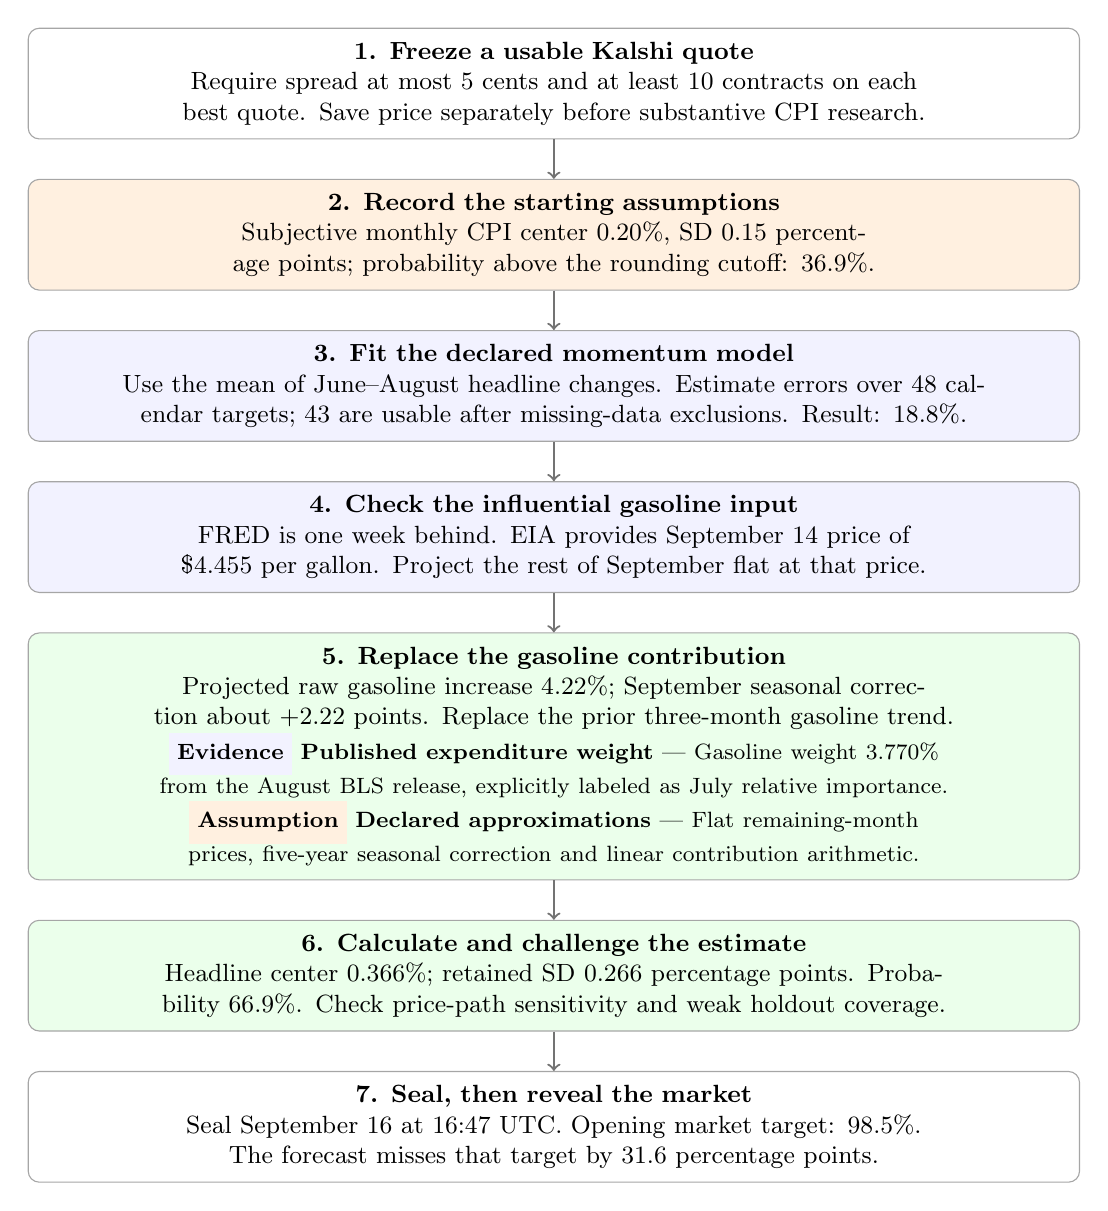
\begin{tikzpicture}[node distance=5mm, every node/.style={font=\small}]
\node[draw=black!35,rounded corners,align=center,text width=13cm,inner sep=5pt,fill=white] (flow0) {\textbf{1. Freeze a usable Kalshi quote}\\ Require spread at most 5 cents and at least 10 contracts on each best quote. Save price separately before substantive CPI research.};
\node[draw=black!35,rounded corners,align=center,text width=13cm,inner sep=5pt,fill=orange!12,below=of flow0] (flow1) {\textbf{2. Record the starting assumptions}\\ Subjective monthly CPI center 0.20\%, SD 0.15 percentage points; probability above the rounding cutoff: 36.9\%.};
\draw[->,thick,draw=black!55] (flow0.south) -- (flow1.north);
\node[draw=black!35,rounded corners,align=center,text width=13cm,inner sep=5pt,fill=blue!5,below=of flow1] (flow2) {\textbf{3. Fit the declared momentum model}\\ Use the mean of June–August headline changes. Estimate errors over 48 calendar targets; 43 are usable after missing-data exclusions. Result: 18.8\%.};
\draw[->,thick,draw=black!55] (flow1.south) -- (flow2.north);
\node[draw=black!35,rounded corners,align=center,text width=13cm,inner sep=5pt,fill=blue!5,below=of flow2] (flow3) {\textbf{4. Check the influential gasoline input}\\ FRED is one week behind. EIA provides September 14 price of \$4.455 per gallon. Project the rest of September flat at that price.};
\draw[->,thick,draw=black!55] (flow2.south) -- (flow3.north);
\node[draw=black!35,rounded corners,align=center,text width=13cm,inner sep=5pt,fill=green!8,below=of flow3] (flow4) {\textbf{5. Replace the gasoline contribution}\\ Projected raw gasoline increase 4.22\%; September seasonal correction about +2.22 points. Replace the prior three-month gasoline trend.\\{\footnotesize\colorbox{blue!5}{\strut\textbf{Evidence}} \textbf{Published expenditure weight} — Gasoline weight 3.770\% from the August BLS release, explicitly labeled as July relative importance.}\\{\footnotesize\colorbox{orange!12}{\strut\textbf{Assumption}} \textbf{Declared approximations} — Flat remaining-month prices, five-year seasonal correction and linear contribution arithmetic.}};
\draw[->,thick,draw=black!55] (flow3.south) -- (flow4.north);
\node[draw=black!35,rounded corners,align=center,text width=13cm,inner sep=5pt,fill=green!8,below=of flow4] (flow5) {\textbf{6. Calculate and challenge the estimate}\\ Headline center 0.366\%; retained SD 0.266 percentage points. Probability 66.9\%. Check price-path sensitivity and weak holdout coverage.};
\draw[->,thick,draw=black!55] (flow4.south) -- (flow5.north);
\node[draw=black!35,rounded corners,align=center,text width=13cm,inner sep=5pt,fill=white,below=of flow5] (flow6) {\textbf{7. Seal, then reveal the market}\\ Seal September 16 at 16:47 UTC. Opening market target: 98.5\%. The forecast misses that target by 31.6 percentage points.};
\draw[->,thick,draw=black!55] (flow5.south) -- (flow6.north);
\end{tikzpicture}
\end{center}
{\small Two model stages within one research pass. The stages are not independent experiments; gasoline information had already been collected when the intermediate momentum result was journaled.}
\clearpage
\section*{\textcolor{epdarkgreen}{The recorded estimates}}
Our initial estimate was a subjective starting model. The momentum stage replaces it with a reproducible historical calculation. The gasoline stage incorporates current information about an influential component. All three estimates were recorded before the market quote was revealed.


\begin{longtable}{>{\raggedright\arraybackslash}p{0.283\linewidth}>{\raggedright\arraybackslash}p{0.283\linewidth}>{\raggedright\arraybackslash}p{0.283\linewidth}}
\textbf{Stage} & \textbf{Probability} & \textbf{Gap below opening midpoint} \\ \hline\endhead
Subjective initial model & 36.9\% & 61.6 percentage points \\
Historical headline momentum & 18.8\% & 79.7 percentage points \\
After current gasoline adjustment & 66.9\% & 31.6 percentage points \\
Opening Kalshi quote & 98–99\%; midpoint 98.5\% & Frozen development target \\
\end{longtable}
\section*{\textcolor{epdarkgreen}{Selection, chronology and liquidity}}
The contract was chosen without viewing its price. Its opening quote was captured at 16:41:57 UTC on September 16. The initial estimate and plan followed at 16:42. The two calculated checkpoints and seal were saved at 16:47. Reveal occurred at 22:28:05 UTC; the later quote was still 98–99\%. The research record does not use intervening information to rewrite the estimate.


The opening best bid had 595.01 contracts and the best ask 2,954.5. There were 5,140.01 bid-side contracts within two cents of the best bid. Both snapshots passed the original ten-contract screen, with unchanged contract terms. This is materially stronger quote depth than the weather examples, although two snapshots do not establish sustained liquidity or market calibration.


This was the same assistant context, with broad macroeconomic information from an earlier Fed case already present. The evaluator store was not inspected before sealing, but no independent context or enforced access barrier was used. Contract thresholds were visible. Research and monetary costs were not separately metered.


\section*{\textcolor{epdarkgreen}{Why the momentum-only estimate was low}}
The fixed baseline averages the preceding three monthly headline CPI changes. Calculated from the downloaded BLS indices, June was −0.4225\%, July +0.0737\% and August +0.3960\%. Their mean is just +0.0157\%. A large June decline therefore continues to pull down this simple September extrapolation.


We compared the same three-month rule with subsequent monthly changes for every target month from September 2022 through August 2026. October 2025 has no published headline index in the downloaded series. That breaks both the target change and several lagged changes, leaving five excluded target months, October 2025 through February 2026. No values were interpolated.


The 43 remaining errors have mean −0.0010 percentage points and sample standard deviation 0.2625. Adding the estimated mean error and its simple sampling-uncertainty allowance gives a baseline center of 0.0147\% and spread of 0.2655 percentage points. Under a normal approximation, that implies an 18.8\% chance above the effective 0.25\% rounding cutoff.


\par{\small Source: \href{https://fred.stlouisfed.org/graph/fredgraph.csv?id=CPIAUCSL,CUSR0000SETB01,CUUR0000SETB01\&cosd=2021-08-01\&coed=2026-08-01}{BLS CPI indices via Federal Reserve Bank of St Louis}}
\par{\small Source: \href{https://www.bls.gov/news.release/cpi.nr0.htm}{BLS August2026 CPI release}}
\par{\small Source: \href{https://www.bls.gov/cpi/seasonal-adjustment/questions-and-answers.htm}{BLS seasonal adjustment FAQ}}
\section*{\textcolor{epdarkgreen}{What the gasoline research changed}}
The FRED gasoline download ended with September 7. Checking EIA’s original spreadsheet found the September 14 all-grades price of \$4.455 per gallon, compared with \$4.295 a week earlier. The primary-source check prevented us from treating a lagging mirror as current.


We carried each weekly price forward to the next observation and the latest price through September 30. The resulting calendar-day averages are \$4.1912 for August and \$4.3681 for projected September, a 4.22\% increase. This is an explicit projection of unobserved days, not a completed monthly observation.


Gasoline normally has a seasonal pattern. Across all five Septembers from 2021 through 2025, the median difference between seasonally adjusted and raw gasoline changes was +2.22 percentage points. Applying that proxy yields about 6.44\% seasonally adjusted gasoline growth. The preceding three-month gasoline trend was −2.88\%.


Replacing that old gasoline contribution with the new one, using the published 3.770\% expenditure weight, adds 0.3515 percentage points to the headline estimate. The August release labels this weight as July relative importance; we preserve that lag explicitly. Rolling it forward approximately gives a 68.0\% sensitivity result rather than the selected 66.9\%. The linear contribution calculation is an approximation to BLS aggregation.


\begin{longtable}{>{\raggedright\arraybackslash}p{0.425\linewidth}>{\raggedright\arraybackslash}p{0.425\linewidth}}
\textbf{Input or calculation} & \textbf{Value} \\ \hline\endhead
August daily-step gasoline average & \$4.1912/gallon \\
Projected September average & \$4.3681/gallon \\
Projected raw gasoline change & +4.22\% \\
Median September seasonal correction & +2.22 percentage points \\
Projected adjusted gasoline change & +6.44\% \\
Prior three-month adjusted gasoline trend & −2.88\% \\
Replacement effect on headline CPI & +0.3515 percentage points \\
\end{longtable}
\par{\small Source: \href{https://www.eia.gov/dnav/pet/hist\_xls/EMM\_EPM0\_PTE\_NUS\_DPGw.xls}{EIA weekly US all-grades all-formulations retail gasoline price history}}
\par{\small Source: \href{https://fred.stlouisfed.org/graph/fredgraph.csv?id=GASALLW\&cosd=2026-07-01\&coed=2026-09-16}{FRED EIA weekly gasoline mirror}}
\par{\small Source: \href{https://www.eia.gov/petroleum/gasdiesel/gas\_proc-methods.php}{EIA retail gasoline survey methodology}}
\par{\small Source: \href{https://fred.stlouisfed.org/graph/fredgraph.csv?id=CPIAUCSL,CUSR0000SETB01,CUUR0000SETB01\&cosd=2021-08-01\&coed=2026-08-01}{BLS CPI indices via Federal Reserve Bank of St Louis}}
\par{\small Source: \href{https://www.bls.gov/news.release/cpi.t01.htm}{BLS CPI August2026 Table1}}
\par{\small Source: \href{https://www.bls.gov/cpi/seasonal-adjustment/questions-and-answers.htm}{BLS seasonal adjustment FAQ}}
\section*{\textcolor{epdarkgreen}{From a CPI point estimate to a probability}}
The final headline center is 0.0147\% + 0.3515\% = 0.3662\%. We retain the baseline model’s 0.2655-percentage-point spread, as declared before retrieval. Assuming normal forecast errors, the chance of an unrounded change at least 0.25\% is 66.9\%. The empirical historical-error version gives 72.1\%. Neither figure is validated calibration for this gasoline-adjusted model.


Keeping an old spread is a modeling choice, not a mathematical requirement. It avoids automatically claiming that additional research increases precision, but it also creates a mismatch: the center uses current gasoline information while the error distribution comes from a model that ignored it. That mismatch is a central limitation of this exercise.


\par{\small Source: \href{https://fred.stlouisfed.org/graph/fredgraph.csv?id=CPIAUCSL,CUSR0000SETB01,CUUR0000SETB01\&cosd=2021-08-01\&coed=2026-08-01}{BLS CPI indices via Federal Reserve Bank of St Louis}}
\par{\small Source: \href{https://www.eia.gov/dnav/pet/hist\_xls/EMM\_EPM0\_PTE\_NUS\_DPGw.xls}{EIA weekly US all-grades all-formulations retail gasoline price history}}
\par{\small Source: \href{https://www.bls.gov/news.release/cpi.t01.htm}{BLS CPI August2026 Table1}}
\par{\small Source: \href{https://assets.kalshi.com/contract\_terms/CPI.pdf}{Kalshi CPI contract terms}}
\par{\small Source: \href{https://www.bls.gov/cpi/seasonal-adjustment/questions-and-answers.htm}{BLS seasonal adjustment FAQ}}
\section*{\textcolor{epdarkgreen}{Sensitivity and a failed calibration check}}
A fixed chronological diagnostic used the first 36 calendar months for fitting and the next 12 for checking. Missing data left only seven usable holdout forecasts. Their RMSE was 0.502 percentage points, and a nominal 90\% interval covered just four of seven outcomes. This is a warning about instability, not evidence that the primary normal approximation is reliable.


Before revealing the market, we also computed a wider-distribution diagnostic using that holdout RMSE as a stand-in for spread. It gives 59.2\%. Seven errors cannot establish a calibrated alternative distribution; we report this to show how much the uncertainty choice matters.


If prices for the unobserved remainder of September are 5\% below or above the flat-price assumption, the primary model gives 53.4–78.5\%. Using each of the five individual historical seasonal corrections gives 65.4–68.1\%. Shifting the final headline center by ±0.05 percentage points gives 59.8–73.4\%. These are assumption sensitivities, not confidence intervals.


\par{\small Source: \href{https://fred.stlouisfed.org/graph/fredgraph.csv?id=CPIAUCSL,CUSR0000SETB01,CUUR0000SETB01\&cosd=2021-08-01\&coed=2026-08-01}{BLS CPI indices via Federal Reserve Bank of St Louis}}
\par{\small Source: \href{https://www.bls.gov/cpi/seasonal-adjustment/questions-and-answers.htm}{BLS seasonal adjustment FAQ}}
\par{\small Source: \href{https://www.eia.gov/dnav/pet/hist\_xls/EMM\_EPM0\_PTE\_NUS\_DPGw.xls}{EIA weekly US all-grades all-formulations retail gasoline price history}}
\par{\small Source: \href{https://www.bls.gov/news.release/cpi.t01.htm}{BLS CPI August2026 Table1}}
\par{\small Source: \href{https://assets.kalshi.com/contract\_terms/CPI.pdf}{Kalshi CPI contract terms}}
\section*{\textcolor{epdarkgreen}{A substantial miss against the chosen development target}}
Kalshi’s opening midpoint was 98.5\%. Our final 66.9\% estimate is 31.6 percentage points lower and 31.1 points below the opening bid. The later midpoint was unchanged. With market agreement as the development criterion, this is a substantial miss even though the gasoline research moved the model closer.


The outcome remains unresolved. Closer agreement is not a resolution score, and these sequential calculations do not identify the causal value of research. We have no basis to claim the market is wrong. Equally, the market quote alone does not tell us which of our inputs or distributional assumptions is responsible for the difference.


A post-reveal Gaussian diagnostic makes the scale explicit. Holding our spread fixed would require a center near 0.826\% to reach 98.5\%. Holding our center fixed would require a spread near 0.054 percentage points. Those are arithmetic descriptions of disagreement, not recommended parameters or new forecasts.


\section*{\textcolor{epdarkgreen}{What should change on the next fresh question}}
Build forecasts for the major CPI components, including shelter/core, food and energy, with dated inputs available at the intended forecast time. Estimate the errors of that complete model using original-release outcomes. A model with a new center and an unrelated old error distribution is not enough.


Make freshness checks explicit: compare mirrored datasets with the primary release and record missing periods. Use the published current seasonal factors where available instead of treating a five-year median as an exact factor. Model the remaining-month gasoline path as a source of uncertainty.


This run uses revised historical CPI indices, a coarse seasonal proxy and a small, weak holdout. It does not establish a calibrated probability. Preserve the sealed 66.9\% result and test the revised process on a new hidden market target rather than tuning this case to 98.5\%.


\section*{\textcolor{epdarkgreen}{About this report}}
This explanation was written at report generation from the recorded research. It does not change the sealed predictions. The complete evidence and calculation records are in the technical appendix.


\clearpage
\appendix
\section{Technical appendix}
Complete records follow. These do not change the assessment above.
\subsection*{\textcolor{epdarkgreen}{Summary}}
Workbench workbench\_1a\hspace{0pt}e01f8856bf4d\hspace{0pt}c5926f: latest estimate 66.9\%; revealed.


\subsection*{\textcolor{epdarkgreen}{Question and resolution}}
\par\noindent\textbf{Created at:} 2026-09-16T16:40:06.267936Z

\par\noindent\textbf{Specification:} \par \par\noindent\textbf{Domain:} economics

\par\noindent\textbf{Event deadline:} 2026-10-14T12:30:00Z

\par\noindent\textbf{Event group:} KXCPI-26SEP

\par\noindent\textbf{Id:} cpi\_sep2026\_above\_0\_2

\par\noindent\textbf{Kind:} real

\par\noindent\textbf{No:} The qualifying expiration value is 0.2\% or lower.

\par\noindent\textbf{Profile:} general

\par\noindent\textbf{Resolution source:} BLS September CPI release, scheduled October14 at08:30EDT; Kalshi KXCPI-26SEP-T0.2 rules and CPI contract PDF control rounding, delays, expiration and fallback. Market close08:25EDT differs from release time.

\par\noindent\textbf{Resolve after:} 2026-10-14T12:31:00Z

\par\noindent\textbf{Text:} Will the published seasonally adjusted monthly CPI-U increase for September 2026 exceed 0.2\%?

\par\noindent\textbf{Void:} Nonbinary discretionary settlement or unresolved ambiguity about a contingency is outside this binary comparison.

\par\noindent\textbf{Yes:} The Kalshi expiration value for September 2026 monthly seasonally adjusted all-items CPI-U, published to one decimal place by BLS, is strictly greater than 0.2\%; ordinarily a reported 0.3\% or higher. The published contract fallback applies if no underlying is released.

\par\noindent\textbf{Version:} 1

\subsection*{\textcolor{epdarkgreen}{Workbench overview}}
\par\noindent\textbf{Case id:} workbench\_1a\hspace{0pt}e01f8856bf4d\hspace{0pt}c5926f

\par\noindent\textbf{State:} revealed

\par\noindent\textbf{Question version:} 1

\par\noindent\textbf{Method:} Inflation momentum plus a declared gasoline contribution adjustment; hidden market comparison

\par\noindent\textbf{Mode:} prospective

\par\noindent\textbf{Latest estimate:} 66.9\%

\par\noindent\textbf{Sealed at:} 2026-09-16T16:47:48.251320Z

\par\noindent\textbf{Market status:} Revealed

\par\noindent\textbf{Opening target captured at:} 2026-09-16T16:41:57.200854Z

\subsection*{\textcolor{epdarkgreen}{Frozen contract and case selection}}
\par\noindent\textbf{Question:} \par \par\noindent\textbf{Created at:} 2026-09-16T16:40:06.267936Z

\par\noindent\textbf{Specification:} \par \par\noindent\textbf{Domain:} economics

\par\noindent\textbf{Event deadline:} 2026-10-14T12:30:00Z

\par\noindent\textbf{Event group:} KXCPI-26SEP

\par\noindent\textbf{Id:} cpi\_sep2026\_above\_0\_2

\par\noindent\textbf{Kind:} real

\par\noindent\textbf{No:} The qualifying expiration value is 0.2\% or lower.

\par\noindent\textbf{Profile:} general

\par\noindent\textbf{Resolution source:} BLS September CPI release, scheduled October14 at08:30EDT; Kalshi KXCPI-26SEP-T0.2 rules and CPI contract PDF control rounding, delays, expiration and fallback. Market close08:25EDT differs from release time.

\par\noindent\textbf{Resolve after:} 2026-10-14T12:31:00Z

\par\noindent\textbf{Text:} Will the published seasonally adjusted monthly CPI-U increase for September 2026 exceed 0.2\%?

\par\noindent\textbf{Void:} Nonbinary discretionary settlement or unresolved ambiguity about a contingency is outside this binary comparison.

\par\noindent\textbf{Yes:} The Kalshi expiration value for September 2026 monthly seasonally adjusted all-items CPI-U, published to one decimal place by BLS, is strictly greater than 0.2\%; ordinarily a reported 0.3\% or higher. The published contract fallback applies if no underlying is released.

\par\noindent\textbf{Version:} 1

\par\noindent\textbf{Contract:} \par \par\noindent\textbf{Event group:} KXCPI-26SEP

\par\noindent\textbf{Market id:} KXCPI-26SEP-T0.2

\par\noindent\textbf{Resolution source:} See frozen Kalshi rules and series contract.

\par\noindent\textbf{Rules:} If the Consumer Price Index (CPI) increases by more than 0.2\% (single-decimal) in September 2026, then the market resolves to Yes.

The market will always close at 8:25 AM ET on the scheduled day of the data release (October 14, 2026). Please note: the Expiration Value is the single-decimal value published at the Source Agency. In the case of a delay in data caused by a federal government shutdown impacting the reliability of the Source Agency, the market’s latest Expiration Date will be extended to the sooner of the release of the Underlying or six months after the end of the government shutdown.

\par\noindent\textbf{Scheduled close:} 2026-10-14T12:25:00Z

\par\noindent\textbf{Title:} Will CPI rise more than 0.2\% in September 2026?

\par\noindent\textbf{Venue:} kalshi

\par\noindent\textbf{Yes description:} Above 0.2\%

\par\noindent\textbf{Selection:} \par \par\noindent\textbf{Contract match rationale:} Monthly all-items CPI-U seasonally adjusted, signed one-decimal change; strictly above0.2. Generic terms and market-specific shutdown/close rules retained. Calculation assumes ordinary release; fallback is not independently modeled.

\par\noindent\textbf{Eligibility rationale:} September is incomplete and its BLS CPI release is scheduled for October14. Select the0.2\% threshold without looking at odds. Require at most5-cent spread and at least10 contracts each side.

\par\noindent\textbf{Market id:} KXCPI-26SEP-T0.2

\par\noindent\textbf{Max spread:} 0.05

\par\noindent\textbf{Method:} Inflation momentum plus a declared gasoline contribution adjustment; hidden market comparison

\par\noindent\textbf{Min contracts each side:} 10

\par\noindent\textbf{Mode:} prospective

\par\noindent\textbf{Question:} \par \par\noindent\textbf{Question id:} cpi\_sep2026\_above\_0\_2

\par\noindent\textbf{Version:} 1

\par\noindent\textbf{Venue:} kalshi

\subsection*{\textcolor{epdarkgreen}{Prediction history}}
Checkpoints are recorded judgments, not necessarily issued forecasts. All timestamps retain their recorded time zones.


\begin{longtable}{>{\raggedright\arraybackslash}p{.27\linewidth}>{\raggedright\arraybackslash}p{.65\linewidth}}
Stage & Initial \\
Probability & 36.9\% \\
Recorded at & 2026-09-16T16:42:39.950330Z \\
Gap to opening market (pp) & -61.56 \\
Squared market error & 0.378912 \\
Step improvement & Not applicable \\
\end{longtable}
\begin{longtable}{>{\raggedright\arraybackslash}p{.27\linewidth}>{\raggedright\arraybackslash}p{.65\linewidth}}
Stage & Research 1: Does current inflation momentum plus observable gasoline pricing put September above the0.25pp unrounded cutoff, and how uncertain is that estimate? \\
Probability & 18.8\% \\
Recorded at & 2026-09-16T16:47:47.928840Z \\
Gap to opening market (pp) & -79.72 \\
Squared market error & 0.635562 \\
Step improvement & -0.256650 \\
\end{longtable}
\begin{longtable}{>{\raggedright\arraybackslash}p{.27\linewidth}>{\raggedright\arraybackslash}p{.65\linewidth}}
Stage & Research 2: Complete the gasoline contribution adjustment specified in the original plan. \\
Probability & 66.9\% \\
Recorded at & 2026-09-16T16:47:48.144970Z \\
Gap to opening market (pp) & -31.58 \\
Squared market error & 0.099747 \\
Step improvement & +0.535815 \\
\end{longtable}
\subsection*{\textcolor{epdarkgreen}{Market comparison}}
Frozen opening midpoint: 98.5\%; bid–ask 98.0\%–99.0\%. Captured 2026-09-16T16:41:57.200854Z.


Later midpoint: 98.5\%; bid–ask 98.0\%–99.0\%. Captured 2026-09-16T22:28:05.744687Z.


Squared market error = (estimate − opening midpoint)². Positive step improvement means closer agreement.


Market agreement is not an outcome score. The later quote is separate from the frozen opening target.


\par\noindent\textbf{Target:} \par \par\noindent\textbf{Ask:} 0.99

\par\noindent\textbf{Ask contracts within 2c:} 2954.5

\par\noindent\textbf{Ask size:} 2954.5

\par\noindent\textbf{Bid:} 0.98

\par\noindent\textbf{Bid contracts within 2c:} 5140.01

\par\noindent\textbf{Bid size:} 595.01

\par\noindent\textbf{Midpoint:} 0.985

\par\noindent\textbf{Spread:} 0.01

\par\noindent\textbf{Target captured at:} 2026-09-16T16:41:57.200854Z

\par\noindent\textbf{Target method:} Opening order-book midpoint, frozen before initial assessment.

\par\noindent\textbf{Net squared error improvement:} 0.279165569248771

\par\noindent\textbf{Followup quote:} \par \par\noindent\textbf{Ask:} 0.99

\par\noindent\textbf{Ask contracts within 2c:} 2500.0

\par\noindent\textbf{Ask size:} 2500.0

\par\noindent\textbf{Bid:} 0.98

\par\noindent\textbf{Bid contracts within 2c:} 52884.22

\par\noindent\textbf{Bid size:} 455.16

\par\noindent\textbf{Midpoint:} 0.985

\par\noindent\textbf{Spread:} 0.01

\par\noindent\textbf{Followup captured at:} 2026-09-16T22:28:05.744687Z

\par\noindent\textbf{Market movement pp:} 0.0

\par\noindent\textbf{Followup error:} Not recorded

\par\noindent\textbf{Contract changed:} No

\par\noindent\textbf{Eligible for blind comparison:} Yes

\par\noindent\textbf{Qualification reasons:} \par None recorded.

\par\noindent\textbf{Limitations:} \par \par\noindent\textit{Item 1.}\par Market agreement is not an outcome score or proof of forecast accuracy.

\par\noindent\textit{Item 2.}\par Step improvements are descriptive; sequential research does not identify causal effects.

\par\noindent\textit{Item 3.}\par Research may include information arriving after the opening target. Inspect market movement and timestamps.

\par\noindent\textit{Item 4.}\par No exposure reported is an agent declaration, not independently verified isolation.

\par\noindent\textit{Item 5.}\par Bid-ask spread is not a confidence interval. Missing follow-up data does not replace the opening target.

\subsection*{\textcolor{epdarkgreen}{Research journal 1: Initial}}
Recorded 2026-09-16T16:42:39.950330Z · pre\_reveal


Entry workbench\_en\hspace{0pt}try\_9b312ecf\hspace{0pt}943747608ac4


\par\noindent\textbf{Assumptions:} \par \par\noindent\textit{Item 1.}\par Ordinary BLS release and usual nearest-tenth rounding

\par\noindent\textit{Item 2.}\par Mean0.20pp, SD0.15pp subjective

\par\noindent\textit{Item 3.}\par No separate probability assigned to shutdown/no-data fallback

\par\noindent\textbf{Evidence refs:} \par None recorded.

\par\noindent\textbf{Probability:} 36.9\%

\par\noindent\textbf{Rationale:} A deliberately simple starting distribution for unrounded monthly headline CPI: normal mean0.20 percentage points and SD0.15 percentage points. Both parameters are subjective macro assumptions, not fitted data. Published single-decimal change must exceed0.2, approximated by unrounded change>=0.25. Broad macro context from the prior Fed example was already present; this is not a fresh-context prior.

\par\noindent\textbf{Research status:} in\_progress

\par\noindent\textbf{Uncertainties:} \par \par\noindent\textit{Item 1.}\par Recent headline and core momentum

\par\noindent\textit{Item 2.}\par Gasoline contribution and seasonal adjustment

\par\noindent\textit{Item 3.}\par Forecast error around a short-run momentum model

\subsection*{\textcolor{epdarkgreen}{Research journal 2: Plan}}
Recorded 2026-09-16T16:42:40.060260Z · pre\_reveal


Entry workbench\_en\hspace{0pt}try\_a0b06e56\hspace{0pt}ffc1457688f0


\par\noindent\textbf{Higher if:} Recent headline momentum and seasonally adjusted gasoline price movement lift the forecast above0.25pp.

\par\noindent\textbf{Lower if:} Underlying momentum is softer or gasoline contributes less than in the preceding three months.

\par\noindent\textbf{Search plan:} Fix this primary model before data: compute unrounded monthly rates from headline CPI-U seasonally adjusted indices. Baseline center is mean June,July,August2026 monthly rates. Estimate bias and residual SD for the same three-prior-month mean rule on all48 target months September2022–August2026, without outcome filtering. Primary spread=s*sqrt(1+1/48); normal residual distribution. First checkpoint is this calibrated momentum model. Then adjust only gasoline: project September US all-grades retail gasoline average using weekly EIA/FRED GASALLW observations available by September16, carrying each Monday observation forward until the next and carrying the last observed price through September30. Compute August and projected September calendar-day averages using the same step rule. Translate raw gasoline change to seasonal-adjusted change by adding median September correction (CPI gasoline SA monthly change minus gasoline NSA change) for all five Septembers2021–2025. Replace the average June–August SA gasoline contribution in the momentum model with this projected contribution, using August2026 BLS gasoline relative importance divided by100. Adjustment=w\_gas*(projected gasoline SA change - mean June–August gasoline SA change). Other components retain their implicit three-month trend. Keep the historical momentum-model spread; do not claim new evidence automatically tightens it. Record a second checkpoint using that fixed calculation. Check BLS release and component table, seasonality definitions, CPI index histories, and EIA weekly retail gasoline definitions. Report empirical residual estimate, a chronological36/12 holdout diagnostic, gasoline remaining-month price sensitivity +/-5\%, seasonal correction across all five individual years, and center shifts +/-0.05pp. No market odds or third-party event probabilities. Do not switch estimators to improve market agreement.

\par\noindent\textbf{Stopping rule:} Complete these specified datasets and two checkpoints. If an input cannot be obtained, retain the last supported model and disclose the missing calculation. No guessing missing weight or seasonality. Minimum36 valid residual targets. Primary historical data may be revised as of today: disclose that they do not recreate original as-released CPI vintages. Stop and seal before revealing price.

\par\noindent\textbf{Uncertainty:} Does current inflation momentum plus observable gasoline pricing put September above the0.25pp unrounded cutoff, and how uncertain is that estimate?

\par\noindent\textbf{Why it matters:} The release threshold is narrow; energy can move headline CPI by several hundredths of a percentage point. A point forecast alone cannot answer the contract.

\subsection*{\textcolor{epdarkgreen}{Research journal 3: Checkpoint}}
Recorded 2026-09-16T16:47:47.928840Z · pre\_reveal


Entry workbench\_en\hspace{0pt}try\_0679ebeb\hspace{0pt}e89a48ab8c88 · Research plan workbench\_en\hspace{0pt}try\_a0b06e56\hspace{0pt}ffc1457688f0


\par\noindent\textbf{Changed assumptions:} \par \par\noindent\textit{Item 1.}\par Replace subjective0.20pp center and0.15pp SD with the predeclared empirical momentum model.

\par\noindent\textit{Item 2.}\par Use actual valid sample size43 in the1+1/n mean-uncertainty term.

\par\noindent\textbf{Evidence refs:} \par \begin{longtable}{>{\raggedright\arraybackslash}p{0.440\linewidth}>{\raggedright\arraybackslash}p{0.440\linewidth}}
Packet id & Record id \\ \hline\endhead
pkt\_320e7ec936174cc70c759ac3 & momentum \\
pkt\_320e7ec936174cc70c759ac3 & holdout \\
\end{longtable}

\par\noindent\textbf{Findings:} Missing October2025 headline data invalidate five targets; no imputation. Recent holdout RMSE is much worse than earlier fitted spread.

\par\noindent\textbf{Limitations:} \par \par\noindent\textit{Item 1.}\par Historical indices are revised; October2025 missing data remove five residual targets.

\par\noindent\textit{Item 2.}\par Gaussian stable residual distribution and three-month momentum are declared modeling assumptions.

\par\noindent\textit{Item 3.}\par Gasoline is a linear contribution approximation; EIA prices, sampling and weights differ from BLS gasoline CPI.

\par\noindent\textit{Item 4.}\par September remainder is projected flat at last observed price; no oil-price, inventory or shock model.

\par\noindent\textit{Item 5.}\par Seasonal correction is five-year September median, not the exact published2026 adjustment factor.

\par\noindent\textit{Item 6.}\par August release reports July relative importance; primary uses its3.770\% lagged weight, with updated-weight sensitivity.

\par\noindent\textit{Item 7.}\par Residual spread is from the momentum model, not a validated gasoline-adjusted model.

\par\noindent\textit{Item 8.}\par Core, shelter, food and other energy keep implicit three-month trend; no separate forward-looking models.

\par\noindent\textit{Item 9.}\par No model for exceptional delayed-release or no-data fallback; ordinary release assumed.

\par\noindent\textit{Item 10.}\par Same assistant context and procedural price separation, not verified independent blinding.

\par\noindent\textit{Item 11.}\par Source retrieval timestamps conservatively use bundle capture time.

\par\noindent\textit{Item 12.}\par The CPI summary/table/FAQ were read through the web tool after direct HTTP403 failures; their relevant facts were transcribed, not saved as complete raw HTML.

\par\noindent\textit{Item 13.}\par Gasoline evidence was collected in the same research pass before the momentum checkpoint; stages isolate calculations, not independent experiments.

\par\noindent\textit{Item 14.}\par Costs and model usage are unmetered.

\par\noindent\textbf{Probability:} 18.8\%

\par\noindent\textbf{Rationale:} First stage of the declared model: use recent three-month headline momentum and43 available historical prediction residuals. Mean0.01472pp and SD0.26552pp give18.78\% above the effective0.25pp threshold. Large June decline depresses the raw trend. This intermediate calculation omits already-collected gasoline evidence; it is not an independent research run.

\par\noindent\textbf{Remaining uncertainties:} \par \par\noindent\textit{Item 1.}\par Gasoline adjustment still to incorporate

\par\noindent\textit{Item 2.}\par Historical regime and revised data

\par\noindent\textit{Item 3.}\par Seven-observation holdout is small and shows poor coverage

\par\noindent\textbf{Sources checked:} \par \par\noindent\textit{Item 1.}\par \href{https://fred.stlouisfed.org/graph/fredgraph.csv?id=CPIAUCSL,CUSR0000SETB01,CUUR0000SETB01\&cosd=2021-08-01\&coed=2026-08-01}{https://fred\hspace{0pt}.stlouisfed.\hspace{0pt}org/graph/fr\hspace{0pt}edgraph.csv?\hspace{0pt}id=CPIAUCSL,\hspace{0pt}CUSR0000SETB\hspace{0pt}01,CUUR0000S\hspace{0pt}ETB01\&cosd=2\hspace{0pt}021-08-01\&co\hspace{0pt}ed=2026-08-0\hspace{0pt}1}

\par\noindent\textit{Item 2.}\par \href{https://www.bls.gov/news.release/cpi.nr0.htm}{https://www.\hspace{0pt}bls.gov/news\hspace{0pt}.release/cpi\hspace{0pt}.nr0.htm}

\par\noindent\textit{Item 3.}\par \href{https://www.bls.gov/cpi/seasonal-adjustment/questions-and-answers.htm}{https://www.\hspace{0pt}bls.gov/cpi/\hspace{0pt}seasonal-adj\hspace{0pt}ustment/ques\hspace{0pt}tions-and-an\hspace{0pt}swers.htm}

\subsection*{\textcolor{epdarkgreen}{Research journal 4: Plan}}
Recorded 2026-09-16T16:47:48.035648Z · pre\_reveal


Entry workbench\_en\hspace{0pt}try\_615f5ca8\hspace{0pt}64c348a5a918


\par\noindent\textbf{Higher if:} Current September gasoline growth exceeds the prior three-month gasoline trend.

\par\noindent\textbf{Lower if:} Remaining-month prices decline or the seasonal contribution is smaller.

\par\noindent\textbf{Search plan:} Use the inputs already collected under the initial pre-data plan and its same formula; this is a continuation, not a claim these inputs are still unseen. Technical clarification: the August BLS release labels3.770\% as July relative importance, so use that published lagged weight and show a rolled-forward August-weight sensitivity. Retain original residual spread for primary model. Add a diagnostic using recent holdout RMSE as an alternative width; do not claim it is calibrated or select it to match the hidden quote.

\par\noindent\textbf{Stopping rule:} Record the gasoline-adjusted model and declared sensitivities, flag the weak uncertainty calibration, then seal.

\par\noindent\textbf{Uncertainty:} Complete the gasoline contribution adjustment specified in the original plan.

\par\noindent\textbf{Why it matters:} The three-month trend averages a sharp June gasoline decline; current gasoline is rising.

\subsection*{\textcolor{epdarkgreen}{Research journal 5: Checkpoint}}
Recorded 2026-09-16T16:47:48.144970Z · pre\_reveal


Entry workbench\_en\hspace{0pt}try\_5ce6787d\hspace{0pt}6f6741b1bac5 · Research plan workbench\_en\hspace{0pt}try\_615f5ca8\hspace{0pt}64c348a5a918


\par\noindent\textbf{Changed assumptions:} \par \par\noindent\textit{Item 1.}\par Replace only the gasoline contribution with observed partial-month prices plus declared flat remainder.

\par\noindent\textit{Item 2.}\par Five-year September median correction approximates gasoline seasonality.

\par\noindent\textit{Item 3.}\par Lagged published weight3.770\%, rather than mistakenly labeling it an August observation.

\par\noindent\textbf{Evidence refs:} \par \begin{longtable}{>{\raggedright\arraybackslash}p{0.440\linewidth}>{\raggedright\arraybackslash}p{0.440\linewidth}}
Packet id & Record id \\ \hline\endhead
pkt\_320e7ec936174cc70c759ac3 & fresh\_gas \\
pkt\_320e7ec936174cc70c759ac3 & gas\_adjustment \\
pkt\_320e7ec936174cc70c759ac3 & final \\
pkt\_320e7ec936174cc70c759ac3 & holdout \\
\end{longtable}

\par\noindent\textbf{Findings:} Primary EIA data extend one week beyond FRED. The implied4.22\% raw gasoline rise plus September seasonal adjustment reverses the backward-looking gasoline drag. Lagged3.770\% weight is transparent; rolled-forward weight sensitivity gives67.97\%.

\par\noindent\textbf{Limitations:} \par \par\noindent\textit{Item 1.}\par Historical indices are revised; October2025 missing data remove five residual targets.

\par\noindent\textit{Item 2.}\par Gaussian stable residual distribution and three-month momentum are declared modeling assumptions.

\par\noindent\textit{Item 3.}\par Gasoline is a linear contribution approximation; EIA prices, sampling and weights differ from BLS gasoline CPI.

\par\noindent\textit{Item 4.}\par September remainder is projected flat at last observed price; no oil-price, inventory or shock model.

\par\noindent\textit{Item 5.}\par Seasonal correction is five-year September median, not the exact published2026 adjustment factor.

\par\noindent\textit{Item 6.}\par August release reports July relative importance; primary uses its3.770\% lagged weight, with updated-weight sensitivity.

\par\noindent\textit{Item 7.}\par Residual spread is from the momentum model, not a validated gasoline-adjusted model.

\par\noindent\textit{Item 8.}\par Core, shelter, food and other energy keep implicit three-month trend; no separate forward-looking models.

\par\noindent\textit{Item 9.}\par No model for exceptional delayed-release or no-data fallback; ordinary release assumed.

\par\noindent\textit{Item 10.}\par Same assistant context and procedural price separation, not verified independent blinding.

\par\noindent\textit{Item 11.}\par Source retrieval timestamps conservatively use bundle capture time.

\par\noindent\textit{Item 12.}\par The CPI summary/table/FAQ were read through the web tool after direct HTTP403 failures; their relevant facts were transcribed, not saved as complete raw HTML.

\par\noindent\textit{Item 13.}\par Gasoline evidence was collected in the same research pass before the momentum checkpoint; stages isolate calculations, not independent experiments.

\par\noindent\textit{Item 14.}\par Costs and model usage are unmetered.

\par\noindent\textbf{Probability:} 66.9\%

\par\noindent\textbf{Rationale:} Apply the originally declared gasoline replacement. Add0.351478pp to the momentum center for final mean0.366199pp; keep SD0.265519pp rather than asserting new evidence justifies tighter uncertainty. Normal tail above0.25pp gives66.9173\%. This model is provisional: poor holdout coverage challenges stationary uncertainty. Using its0.50164pp RMSE as an alternative width gives59.16\%, a diagnostic not a fitted replacement.

\par\noindent\textbf{Remaining uncertainties:} \par \par\noindent\textit{Item 1.}\par Remaining-month prices and shocks

\par\noindent\textit{Item 2.}\par EIA-to-BLS gasoline mapping and exact seasonal factor

\par\noindent\textit{Item 3.}\par Other CPI components retain backward-looking trends

\par\noindent\textit{Item 4.}\par Historical residual spread may not describe the current regime

\par\noindent\textbf{Sources checked:} \par \par\noindent\textit{Item 1.}\par \href{https://fred.stlouisfed.org/graph/fredgraph.csv?id=CPIAUCSL,CUSR0000SETB01,CUUR0000SETB01\&cosd=2021-08-01\&coed=2026-08-01}{https://fred\hspace{0pt}.stlouisfed.\hspace{0pt}org/graph/fr\hspace{0pt}edgraph.csv?\hspace{0pt}id=CPIAUCSL,\hspace{0pt}CUSR0000SETB\hspace{0pt}01,CUUR0000S\hspace{0pt}ETB01\&cosd=2\hspace{0pt}021-08-01\&co\hspace{0pt}ed=2026-08-0\hspace{0pt}1}

\par\noindent\textit{Item 2.}\par \href{https://www.bls.gov/news.release/cpi.nr0.htm}{https://www.\hspace{0pt}bls.gov/news\hspace{0pt}.release/cpi\hspace{0pt}.nr0.htm}

\par\noindent\textit{Item 3.}\par \href{https://www.bls.gov/news.release/cpi.t01.htm}{https://www.\hspace{0pt}bls.gov/news\hspace{0pt}.release/cpi\hspace{0pt}.t01.htm}

\par\noindent\textit{Item 4.}\par \href{https://www.eia.gov/dnav/pet/hist\_xls/EMM\_EPM0\_PTE\_NUS\_DPGw.xls}{https://www.\hspace{0pt}eia.gov/dnav\hspace{0pt}/pet/hist\_xl\hspace{0pt}s/EMM\_EPM0\_P\hspace{0pt}TE\_NUS\_DPGw.\hspace{0pt}xls}

\par\noindent\textit{Item 5.}\par \href{https://fred.stlouisfed.org/graph/fredgraph.csv?id=GASALLW\&cosd=2026-07-01\&coed=2026-09-16}{https://fred\hspace{0pt}.stlouisfed.\hspace{0pt}org/graph/fr\hspace{0pt}edgraph.csv?\hspace{0pt}id=GASALLW\&c\hspace{0pt}osd=2026-07-\hspace{0pt}01\&coed=2026\hspace{0pt}-09-16}

\par\noindent\textit{Item 6.}\par \href{https://www.bls.gov/cpi/seasonal-adjustment/questions-and-answers.htm}{https://www.\hspace{0pt}bls.gov/cpi/\hspace{0pt}seasonal-adj\hspace{0pt}ustment/ques\hspace{0pt}tions-and-an\hspace{0pt}swers.htm}

\par\noindent\textit{Item 7.}\par \href{https://www.eia.gov/petroleum/gasdiesel/gas\_proc-methods.php}{https://www.\hspace{0pt}eia.gov/petr\hspace{0pt}oleum/gasdie\hspace{0pt}sel/gas\_proc\hspace{0pt}-methods.php}

\par\noindent\textit{Item 8.}\par \href{https://assets.kalshi.com/contract\_terms/CPI.pdf}{https://asse\hspace{0pt}ts.kalshi.co\hspace{0pt}m/contract\_t\hspace{0pt}erms/CPI.pdf}

\subsection*{\textcolor{epdarkgreen}{Research journal 6: Finish}}
Recorded 2026-09-16T16:47:48.251320Z · pre\_reveal


Entry workbench\_en\hspace{0pt}try\_cbde94ad\hspace{0pt}40694d69b776


\par\noindent\textbf{Exposure notes:} No CPI market price or outside event probability observed before seal. Same existing assistant context, including prior Fed-study macro context. Evaluator file store not inspected; no enforced isolation.

\par\noindent\textbf{Market exposure:} none

\par\noindent\textbf{Outcome status:} unresolved

\par\noindent\textbf{Stopping reason:} Completed the fixed momentum model, primary-source gasoline update, seasonal proxy, lagged-weight clarification and sensitivity diagnostics. Report a provisional estimate with weak uncertainty validation; further method changes belong on a fresh target.

\subsection*{\textcolor{epdarkgreen}{Research journal 7: Reflection}}
Recorded 2026-09-16T22:29:38.890291Z · post\_reveal


Entry workbench\_en\hspace{0pt}try\_1bca3421\hspace{0pt}c6164ef2a880


\par\noindent\textbf{Next method change:} On a fresh hidden target, use a component model with explicit food, shelter/core and energy forecasts. Calibrate the complete model on dated historical partial-month inputs and first-release outcomes, not revised data or baseline-model errors. Add a source-freshness requirement comparing mirrors with the primary release. Use current published seasonal factors if available, and record reasons for exceptional-release assumptions. Do not choose a smaller SD merely to fit this revealed98.5\% quote. Under the user’s market-target criterion, this run is a substantial miss despite the useful gasoline update.

\par\noindent\textbf{What did not:} The sealed forecast remains31.6 points below the opening midpoint. Three-month headline momentum is distorted by large changing gasoline contributions; its historical residual variance is not the conditional uncertainty of the gasoline-adjusted model. Recent holdout coverage was poor. We did not validate the full adjusted model, model other CPI components forward, use exact2026 seasonal factors, or forecast the remaining gasoline-price path. These are concrete shortcomings, not evidence that Kalshi is wrong.

\par\noindent\textbf{What helped:} The primary EIA workbook supplied a week missing from FRED, and explicit gasoline seasonality/contribution arithmetic changed the estimate from18.8\% momentum-only to66.9\%. This moved markedly closer to the opening98.5\% midpoint. Quote depth passed the predeclared screen without relaxing it.

\subsection*{\textcolor{epdarkgreen}{Model and calculation}}
No structured model artifact was attached to this case. The recorded rationales and assumptions above are the available model description. Supplemental files, if supplied, are identified separately below.


\subsection*{\textcolor{epdarkgreen}{Limitations and research cost}}
\par\noindent\textbf{Case limitations:} \par \par\noindent\textit{Item 1.}\par Prices are separated from this project, not protected by an operating-system sandbox.

\par\noindent\textit{Item 2.}\par Selection checks spread and top-of-book size only; neither establishes market accuracy.

\par\noindent\textit{Item 3.}\par The agent must verify the event is still unknown; an open market alone cannot establish this.

\par\noindent\textbf{Reported usage:} \par None recorded.

\par\noindent\textbf{Usage note:} Usage is agent-reported. Missing usage is unmetered, not zero; partial records are not a total.

\subsection*{\textcolor{epdarkgreen}{Supplemental model or research file: calculation.json}}
Supplied at report generation. This is not automatically part of the sealed research record; its hash can be compared with a previously recorded commitment. No code in this file was executed.


\par\noindent\textbf{Name:} calculation.json

\par\noindent\textbf{Sha256:} f6eee597d3fd\hspace{0pt}622fe665ef63\hspace{0pt}78b253d61c11\hspace{0pt}3493f8f60002\hspace{0pt}774cd5318ddf\hspace{0pt}b2dd

\par\noindent\textbf{Provenance:} report\_time\_attachment

\par\noindent\textbf{Content:} \par \par\noindent\textbf{Units:} Monthly inflation percentage points, not fractions. Probability is a fraction.

\par\noindent\textbf{Initial probability:} 0.36944134018176367

\par\noindent\textbf{N:} 43

\par\noindent\textbf{Pairs:} \par \begin{longtable}{>{\raggedright\arraybackslash}p{0.220\linewidth}>{\raggedright\arraybackslash}p{0.220\linewidth}>{\raggedright\arraybackslash}p{0.220\linewidth}>{\raggedright\arraybackslash}p{0.220\linewidth}}
Month & Actual change pp & Three month forecast pp & Error pp \\ \hline\endhead
2022-09-01 & 0.42426727482827165 & 0.434525283831666 & -0.010258009003394353 \\
2022-10-01 & 0.5594754832984217 & 0.15724704256090036 & 0.4022284407375213 \\
2022-11-01 & 0.2614032556282231 & 0.34871134654108626 & -0.08730809091286318 \\
2022-12-01 & 0.01539563433359259 & 0.4150486712516388 & -0.3996530369180462 \\
2023-01-01 & 0.5314022594635093 & 0.27875812442007913 & 0.25264413504343014 \\
2023-02-01 & 0.3428533386591992 & 0.269400383141775 & 0.0734529555174242 \\
2023-03-01 & 0.12307181953890023 & 0.29655041081876704 & -0.1734785912798668 \\
2023-04-01 & 0.3392739405144063 & 0.33244247255386955 & 0.006831467960536741 \\
2023-05-01 & 0.1614687381333635 & 0.26839969957083526 & -0.10693096143747177 \\
2023-06-01 & 0.224175331482801 & 0.20793816606222335 & 0.016237165420577654 \\
2023-07-01 & 0.1957146710348745 & 0.24163933671019025 & -0.04592466567531575 \\
2023-08-01 & 0.4835707415079771 & 0.19378624688367965 & 0.28978449462429745 \\
2023-09-01 & 0.3900915440960384 & 0.3011535813418842 & 0.08893796275415422 \\
2023-10-01 & 0.13668493471667986 & 0.3564589855462967 & -0.21977405082961682 \\
2023-11-01 & 0.14689823722116024 & 0.33678240677356513 & -0.1898841695524049 \\
2023-12-01 & 0.1924399963653789 & 0.22455823867795952 & -0.03211824231258062 \\
2024-01-01 & 0.30996854969052023 & 0.15867438943440634 & 0.1512941602561139 \\
2024-02-01 & 0.40975401843086345 & 0.21643559442568647 & 0.193318424005177 \\
2024-03-01 & 0.4431338373525273 & 0.3040541881622542 & 0.1390796491902731 \\
2024-04-01 & 0.21706766556210955 & 0.387618801824637 & -0.17055113626252744 \\
2024-05-01 & 0.04855873210594108 & 0.3566518404485001 & -0.30809310834255904 \\
2024-06-01 & -0.041829647960411886 & 0.23625341167352598 & -0.27808305963393787 \\
2024-07-01 & 0.16770805381991494 & 0.07459891656921291 & 0.09310913725070202 \\
2024-08-01 & 0.1572221743858515 & 0.05814571265514804 & 0.09907646173070347 \\
2024-09-01 & 0.2133336729690294 & 0.09436686008178485 & 0.11896681288724453 \\
2024-10-01 & 0.2856398459641696 & 0.17942130039159862 & 0.10621854557257096 \\
2024-11-01 & 0.28419261732848256 & 0.21873189777301683 & 0.06546071955546573 \\
2024-12-01 & 0.3399383308901438 & 0.26105537875389384 & 0.07888295213624996 \\
2025-01-01 & 0.42726162139017365 & 0.3032569313942653 & 0.12400468999590836 \\
2025-02-01 & 0.22510589068882592 & 0.3504641898696 & -0.12535829918077407 \\
2025-03-01 & 0.03315826188146076 & 0.33076861432304777 & -0.297610352441587 \\
2025-04-01 & 0.16167112278562268 & 0.22850859132015344 & -0.06683746853453076 \\
2025-05-01 & 0.09928130327003792 & 0.13997842511863645 & -0.04069712184859853 \\
2025-06-01 & 0.2541949971929469 & 0.09803689597904046 & 0.15615810121390644 \\
2025-07-01 & 0.22835098853577485 & 0.17171580774953585 & 0.056635180786239 \\
2025-08-01 & 0.3482644202266627 & 0.19394242966625322 & 0.1543219905604095 \\
2025-09-01 & 0.2950901819104068 & 0.27693680198512816 & 0.018153379925278657 \\
2026-03-01 & 0.8651438343614481 & 0.24521138428212166 & 0.6199324500793265 \\
2026-04-01 & 0.6400377846336402 & 0.43432985283440306 & 0.2057079317992372 \\
2026-05-01 & 0.47291422864139676 & 0.5907282310682641 & -0.11781400242686735 \\
2026-06-01 & -0.42248165303806484 & 0.6593652825454951 & -1.08184693558356 \\
2026-07-01 & 0.07366914435544825 & 0.2301567867456574 & -0.15648764239020915 \\
2026-08-01 & 0.3960181843858157 & 0.04136723998626005 & 0.35465094439955563 \\
\end{longtable}

\par\noindent\textbf{Excluded:} \par \begin{longtable}{>{\raggedright\arraybackslash}p{0.440\linewidth}>{\raggedright\arraybackslash}p{0.440\linewidth}}
Month & Reason \\ \hline\endhead
2025-10-01 & Missing target or one of three lagged monthly changes; no interpolation. \\
2025-11-01 & Missing target or one of three lagged monthly changes; no interpolation. \\
2025-12-01 & Missing target or one of three lagged monthly changes; no interpolation. \\
2026-01-01 & Missing target or one of three lagged monthly changes; no interpolation. \\
2026-02-01 & Missing target or one of three lagged monthly changes; no interpolation. \\
\end{longtable}

\par\noindent\textbf{Recent headline changes pp:} \par \par\noindent\textbf{2026-06:} -0.42248165303806484

\par\noindent\textbf{2026-07:} 0.07366914435544825

\par\noindent\textbf{2026-08:} 0.3960181843858157

\par\noindent\textbf{Raw momentum center pp:} 0.015735225234399703

\par\noindent\textbf{Mean residual pp:} -0.0010144370038234426

\par\noindent\textbf{Sample residual sd pp:} 0.26248394571848377

\par\noindent\textbf{Predictive sd pp:} 0.2655185430145959

\par\noindent\textbf{Momentum center pp:} 0.01472078823057626

\par\noindent\textbf{Momentum probability:} 0.1877785433996466

\par\noindent\textbf{Holdout:} \par \par\noindent\textbf{Train n:} 36

\par\noindent\textbf{Test n:} 7

\par\noindent\textbf{Train bias pp:} 0.0031689745286897367

\par\noindent\textbf{Train sd pp:} 0.17983254839871332

\par\noindent\textbf{Raw rmse pp:} 0.5016401879054787

\par\noindent\textbf{Corrected rmse pp:} 0.5017924959255947

\par\noindent\textbf{Nominal90 coverage:} 0.5714285714285714

\par\noindent\textbf{Halfwidth pp:} 0.2998783876611614

\par\noindent\textbf{Qualification:} Fixed first36/last12 calendar months; missing data reduce valid holdout to seven. Revised-vintage diagnostic, not original-release validation.

\par\noindent\textbf{Gasoline:} \par \par\noindent\textbf{Latest observation:} 2026-09-14

\par\noindent\textbf{Latest price:} 4.455

\par\noindent\textbf{August daily step average:} 4.191193548387097

\par\noindent\textbf{September projected daily step average:} 4.3680666666666665

\par\noindent\textbf{Raw projected change pct:} 4.22011334569925

\par\noindent\textbf{Seasonal corrections:} \par \begin{longtable}{>{\raggedright\arraybackslash}p{0.220\linewidth}>{\raggedright\arraybackslash}p{0.220\linewidth}>{\raggedright\arraybackslash}p{0.220\linewidth}>{\raggedright\arraybackslash}p{0.220\linewidth}}
Year & Sa change pct & Nsa change pct & Correction pp \\ \hline\endhead
2021 & 2.394040566415989 & 0.32078083100257615 & 2.073259735413413 \\
2022 & -3.7216736795961047 & -5.644117925489045 & 1.9224442458929403 \\
2023 & 2.7899203277098383 & 0.5679879161609502 & 2.221932411548888 \\
2024 & -2.8270912930686842 & -5.06482727606401 & 2.237735982995326 \\
2025 & 3.5936542621123335 & 1.1464169600294838 & 2.4472373020828497 \\
\end{longtable}

\par\noindent\textbf{Median seasonal correction pp:} 2.221932411548888

\par\noindent\textbf{Projected sa change pct:} 6.442045757248138

\par\noindent\textbf{Recent three month sa change pct:} -2.8809794370296

\par\noindent\textbf{Weight fraction:} 0.0377

\par\noindent\textbf{Weight reference month:} 2026-07

\par\noindent\textbf{Headline adjustment pp:} 0.3514780498242707

\par\noindent\textbf{Final center pp:} 0.366198838054847

\par\noindent\textbf{Final probability:} 0.6691726825804136

\par\noindent\textbf{Empirical residual probability:} 0.7209302325581395

\par\noindent\textbf{Remaining month gas sensitivity:} \par \begin{longtable}{>{\raggedright\arraybackslash}p{0.293\linewidth}>{\raggedright\arraybackslash}p{0.293\linewidth}>{\raggedright\arraybackslash}p{0.293\linewidth}}
Future price shift & Center pp & Probability \\ \hline\endhead
-0.05 & 0.2726952822119506 & 0.5340582419535114 \\
0 & 0.366198838054847 & 0.6691726825804136 \\
0.05 & 0.4597023938977433 & 0.7851731442463052 \\
\end{longtable}

\par\noindent\textbf{Seasonal sensitivity:} \par \begin{longtable}{>{\raggedright\arraybackslash}p{0.293\linewidth}>{\raggedright\arraybackslash}p{0.293\linewidth}>{\raggedright\arraybackslash}p{0.293\linewidth}}
Year & Center pp & Probability \\ \hline\endhead
2021 & 0.3605938781645396 & 0.6614853626020221 \\
2022 & 0.35490813420961775 & 0.6536178984474103 \\
2023 & 0.366198838054847 & 0.6691726825804136 \\
2024 & 0.3667946326983777 & 0.6699857193865957 \\
2025 & 0.3746928324279773 & 0.6806867526595564 \\
\end{longtable}

\par\noindent\textbf{Center sensitivity:} \par \begin{longtable}{>{\raggedright\arraybackslash}p{0.440\linewidth}>{\raggedright\arraybackslash}p{0.440\linewidth}}
Shift pp & Probability \\ \hline\endhead
-0.05 & 0.5984430120545602 \\
0 & 0.6691726825804136 \\
0.05 & 0.7343230507843395 \\
\end{longtable}

\par\noindent\textbf{Rolled weight sensitivity:} \par \par\noindent\textbf{Weight fraction:} 0.038532934906495134

\par\noindent\textbf{Probability:} 0.6797058036818716

\par\noindent\textbf{Label:} Approximate August weight rolled forward with NSA relative changes; not selected primary.

\par\noindent\textbf{Limitations:} \par \par\noindent\textit{Item 1.}\par Historical indices are revised; October2025 missing data remove five residual targets.

\par\noindent\textit{Item 2.}\par Gaussian stable residual distribution and three-month momentum are declared modeling assumptions.

\par\noindent\textit{Item 3.}\par Gasoline is a linear contribution approximation; EIA prices, sampling and weights differ from BLS gasoline CPI.

\par\noindent\textit{Item 4.}\par September remainder is projected flat at last observed price; no oil-price, inventory or shock model.

\par\noindent\textit{Item 5.}\par Seasonal correction is five-year September median, not the exact published2026 adjustment factor.

\par\noindent\textit{Item 6.}\par August release reports July relative importance; primary uses its3.770\% lagged weight, with updated-weight sensitivity.

\par\noindent\textit{Item 7.}\par Residual spread is from the momentum model, not a validated gasoline-adjusted model.

\par\noindent\textit{Item 8.}\par Core, shelter, food and other energy keep implicit three-month trend; no separate forward-looking models.

\par\noindent\textit{Item 9.}\par No model for exceptional delayed-release or no-data fallback; ordinary release assumed.

\par\noindent\textit{Item 10.}\par Same assistant context and procedural price separation, not verified independent blinding.

\par\noindent\textbf{Raw sha256:} \par \par\noindent\textbf{Bls weight.json:} 2dd141c4a1d4\hspace{0pt}c470a33721ea\hspace{0pt}9cf2e7d0d438\hspace{0pt}8391cb4d176d\hspace{0pt}8d3b4a28773c\hspace{0pt}bfdb

\par\noindent\textbf{Contract.pdf:} 2317b1d8e823\hspace{0pt}082b409f6ff3\hspace{0pt}415fb135804d\hspace{0pt}9682681f9f92\hspace{0pt}f640b3681b29\hspace{0pt}a872

\par\noindent\textbf{Contract.txt:} 72aa0a88d670\hspace{0pt}87b387a4294f\hspace{0pt}17eee41eaaa1\hspace{0pt}aef6a01caa9f\hspace{0pt}7490286cfb04\hspace{0pt}7bdf

\par\noindent\textbf{Cpi indices.csv:} beba624d05a9\hspace{0pt}b51060819516\hspace{0pt}32efe5b41047\hspace{0pt}fef956ac1b0a\hspace{0pt}d59246f68f9c\hspace{0pt}b0dc

\par\noindent\textbf{Eia gasoline weekly.xls:} a6f774ea70a2\hspace{0pt}b0f32db48e42\hspace{0pt}55ba5ff7fe7d\hspace{0pt}99c106320d22\hspace{0pt}683ab5a9d64e\hspace{0pt}7aac

\par\noindent\textbf{Eia method.html:} 6bb5835afeb9\hspace{0pt}681731b884f7\hspace{0pt}3ea6c96b5471\hspace{0pt}5eebaadbd319\hspace{0pt}addcaeb73ab3\hspace{0pt}41f4

\par\noindent\textbf{Gasoline primary.csv:} b8ae43b752de\hspace{0pt}f92b626764ef\hspace{0pt}54112762625b\hspace{0pt}6e01656edc0f\hspace{0pt}7fa8acf28ddd\hspace{0pt}2b5b

\par\noindent\textbf{Gasoline weekly.csv:} 52f2068c19c0\hspace{0pt}92b36af9e3a5\hspace{0pt}0f60ca13da9d\hspace{0pt}02b86a735bc1\hspace{0pt}c84cdd68e40a\hspace{0pt}be57

\par\noindent\textbf{Series.json:} f5c410bc20a2\hspace{0pt}80d5fc14e33d\hspace{0pt}1b028777a3a8\hspace{0pt}8aa6a955938e\hspace{0pt}eee03cc48186\hspace{0pt}6e60

\subsection*{\textcolor{epdarkgreen}{Finding: pkt\_320e7ec9\hspace{0pt}36174cc70c75\hspace{0pt}9ac3:momentu\hspace{0pt}m}}
Sources: [1], [2], [3]


\par\noindent\textbf{Claim:} Fixed three-month momentum center 0.015735pp; mean residual -0.001014pp;43 valid residual targets out of48, excludingOct\hspace{0pt}ober2025–Feb\hspace{0pt}ruary2026 due to the missing CPI index. SD0.265519pp gives18.777854\% above0.25pp.

\par\noindent\textbf{Claim type:} inference

\par\noindent\textbf{Entity ids:} \par None recorded.

\par\noindent\textbf{Id:} momentum

\par\noindent\textbf{Observed at:} 2026-09-16T1\hspace{0pt}6:47:47.7441\hspace{0pt}96+00:00

\par\noindent\textbf{Provenance:} \par \par\noindent\textbf{Adapter:} vorhersage.r\hspace{0pt}esearch\_bund\hspace{0pt}le.v1

\par\noindent\textbf{Value:} Not recorded

\subsection*{\textcolor{epdarkgreen}{Finding: pkt\_320e7ec9\hspace{0pt}36174cc70c75\hspace{0pt}9ac3:holdout}}
Sources: [1], [3]


\par\noindent\textbf{Claim:} Fixed36-month training and12-calendar-month holdout leave36 and7 valid observations. Held-out RMSE0.5016pp; bias correction does not improve it. Nominal90\% interval covers4/7=57.1\%. This raises a calibration/regime warning, not a validated accuracy claim.

\par\noindent\textbf{Claim type:} inference

\par\noindent\textbf{Entity ids:} \par None recorded.

\par\noindent\textbf{Id:} holdout

\par\noindent\textbf{Observed at:} 2026-09-16T1\hspace{0pt}6:47:47.7441\hspace{0pt}96+00:00

\par\noindent\textbf{Provenance:} \par \par\noindent\textbf{Adapter:} vorhersage.r\hspace{0pt}esearch\_bund\hspace{0pt}le.v1

\par\noindent\textbf{Value:} Not recorded

\subsection*{\textcolor{epdarkgreen}{Finding: pkt\_320e7ec9\hspace{0pt}36174cc70c75\hspace{0pt}9ac3:fresh\_g\hspace{0pt}as}}
Sources: [4], [5], [6]


\par\noindent\textbf{Claim:} FRED stopped September7; the EIA workbook adds September14 all-grades\$4.455/gal. Carrying the last price through month-end gives a September average\$4.3681 versus August\$4.1912, a4.2201\% increase.

\par\noindent\textbf{Claim type:} inference

\par\noindent\textbf{Entity ids:} \par None recorded.

\par\noindent\textbf{Id:} fresh\_gas

\par\noindent\textbf{Observed at:} 2026-09-16T1\hspace{0pt}6:47:47.7441\hspace{0pt}96+00:00

\par\noindent\textbf{Provenance:} \par \par\noindent\textbf{Adapter:} vorhersage.r\hspace{0pt}esearch\_bund\hspace{0pt}le.v1

\par\noindent\textbf{Value:} Not recorded

\subsection*{\textcolor{epdarkgreen}{Finding: pkt\_320e7ec9\hspace{0pt}36174cc70c75\hspace{0pt}9ac3:gas\_adj\hspace{0pt}ustment}}
Sources: [1], [7], [4], [3]


\par\noindent\textbf{Claim:} September seasonal correction from all five2021–2025 Septembers has median+2.2219 percentage points. Projected gasoline SA growth6.4420\% replaces the prior three-month average-2.8810\%; a3.770\% lagged weight adds0.351478pp to headline prediction. Linear contribution is approximate.

\par\noindent\textbf{Claim type:} inference

\par\noindent\textbf{Entity ids:} \par None recorded.

\par\noindent\textbf{Id:} gas\_adjustment

\par\noindent\textbf{Observed at:} 2026-09-16T1\hspace{0pt}6:47:47.7441\hspace{0pt}96+00:00

\par\noindent\textbf{Provenance:} \par \par\noindent\textbf{Adapter:} vorhersage.r\hspace{0pt}esearch\_bund\hspace{0pt}le.v1

\par\noindent\textbf{Value:} Not recorded

\subsection*{\textcolor{epdarkgreen}{Finding: pkt\_320e7ec9\hspace{0pt}36174cc70c75\hspace{0pt}9ac3:final}}
Sources: [1], [4], [7], [8]


\par\noindent\textbf{Claim:} Primary final headline center 0.366199pp and retained momentum-model SD0.265519pp imply66.917268\% probability. Remaining-month gasoline prices +/-5\% give53.41–78.52\%. Calculation SHA256 f6eee597d3fd\hspace{0pt}622fe665ef63\hspace{0pt}78b253d61c11\hspace{0pt}3493f8f60002\hspace{0pt}774cd5318ddf\hspace{0pt}b2dd

\par\noindent\textbf{Claim type:} inference

\par\noindent\textbf{Entity ids:} \par None recorded.

\par\noindent\textbf{Id:} final

\par\noindent\textbf{Observed at:} 2026-09-16T1\hspace{0pt}6:47:47.7441\hspace{0pt}96+00:00

\par\noindent\textbf{Provenance:} \par \par\noindent\textbf{Adapter:} vorhersage.r\hspace{0pt}esearch\_bund\hspace{0pt}le.v1

\par\noindent\textbf{Value:} Not recorded

\subsection*{\textcolor{epdarkgreen}{Source [1]: BLS CPI indices via Federal Reserve Bank of St Louis}}
\par\noindent\textbf{Excerpt:} Downloaded headline SA and gasoline SA/NSA monthly index levels through August2026. October2025 headline is missing. The calculation filters observations to the predeclared window.

\par\noindent\textbf{Excerpt kind:} paraphrase

\par\noindent\textbf{Id:} indices

\par\noindent\textbf{Retrieved at:} 2026-09-16T1\hspace{0pt}6:47:47.7441\hspace{0pt}96+00:00

\par\noindent\textbf{Title:} BLS CPI indices via Federal Reserve Bank of St Louis

\par\noindent\textbf{Url:} \href{https://fred.stlouisfed.org/graph/fredgraph.csv?id=CPIAUCSL,CUSR0000SETB01,CUUR0000SETB01\&cosd=2021-08-01\&coed=2026-08-01}{https://fred\hspace{0pt}.stlouisfed.\hspace{0pt}org/graph/fr\hspace{0pt}edgraph.csv?\hspace{0pt}id=CPIAUCSL,\hspace{0pt}CUSR0000SETB\hspace{0pt}01,CUUR0000S\hspace{0pt}ETB01\&cosd=2\hspace{0pt}021-08-01\&co\hspace{0pt}ed=2026-08-0\hspace{0pt}1}

\subsection*{\textcolor{epdarkgreen}{Source [2]: BLS August2026 CPI release}}
\par\noindent\textbf{Excerpt:} Published September11. Headline monthly changes were -0.4\%,+0.1\%,+0.4\% for June–August; August core rose0.3\%. Gasoline increased3.9\% in August. September release scheduled October14. Seasonal data are revised annually.

\par\noindent\textbf{Excerpt kind:} paraphrase

\par\noindent\textbf{Id:} bls

\par\noindent\textbf{Published at:} 2026-09-11T12:30:00Z

\par\noindent\textbf{Retrieved at:} 2026-09-16T1\hspace{0pt}6:47:47.7441\hspace{0pt}96+00:00

\par\noindent\textbf{Title:} BLS August2026 CPI release

\par\noindent\textbf{Url:} \href{https://www.bls.gov/news.release/cpi.nr0.htm}{https://www.\hspace{0pt}bls.gov/news\hspace{0pt}.release/cpi\hspace{0pt}.nr0.htm}

\subsection*{\textcolor{epdarkgreen}{Source [3]: BLS seasonal adjustment FAQ}}
\par\noindent\textbf{Excerpt:} Seasonality removes recurring calendar effects. Factors and historical seasonally adjusted series are revised. October2025 was unavailable for many series because of the funding lapse; special methods were used in seasonal estimation.

\par\noindent\textbf{Excerpt kind:} paraphrase

\par\noindent\textbf{Id:} seasonal

\par\noindent\textbf{Retrieved at:} 2026-09-16T1\hspace{0pt}6:47:47.7441\hspace{0pt}96+00:00

\par\noindent\textbf{Title:} BLS seasonal adjustment FAQ

\par\noindent\textbf{Url:} \href{https://www.bls.gov/cpi/seasonal-adjustment/questions-and-answers.htm}{https://www.\hspace{0pt}bls.gov/cpi/\hspace{0pt}seasonal-adj\hspace{0pt}ustment/ques\hspace{0pt}tions-and-an\hspace{0pt}swers.htm}

\subsection*{\textcolor{epdarkgreen}{Source [4]: EIA weekly US all-grades all-formulations retail gasoline price history}}
\par\noindent\textbf{Excerpt:} Latest observed Monday September14 price is\$4.455/gal, versus\$4.295 September7 and\$4.207 August31. Archived original workbook and extracted recent rows.

\par\noindent\textbf{Excerpt kind:} paraphrase

\par\noindent\textbf{Id:} eia

\par\noindent\textbf{Retrieved at:} 2026-09-16T1\hspace{0pt}6:47:47.7441\hspace{0pt}96+00:00

\par\noindent\textbf{Title:} EIA weekly US all-grades all-formulations retail gasoline price history

\par\noindent\textbf{Url:} \href{https://www.eia.gov/dnav/pet/hist\_xls/EMM\_EPM0\_PTE\_NUS\_DPGw.xls}{https://www.\hspace{0pt}eia.gov/dnav\hspace{0pt}/pet/hist\_xl\hspace{0pt}s/EMM\_EPM0\_P\hspace{0pt}TE\_NUS\_DPGw.\hspace{0pt}xls}

\subsection*{\textcolor{epdarkgreen}{Source [5]: FRED EIA weekly gasoline mirror}}
\par\noindent\textbf{Excerpt:} Downloaded series ended September7 at\$4.295. Primary EIA workbook supplies the missing September14 observation; do not treat the mirror as current.

\par\noindent\textbf{Excerpt kind:} paraphrase

\par\noindent\textbf{Id:} fredgas

\par\noindent\textbf{Retrieved at:} 2026-09-16T1\hspace{0pt}6:47:47.7441\hspace{0pt}96+00:00

\par\noindent\textbf{Title:} FRED EIA weekly gasoline mirror

\par\noindent\textbf{Url:} \href{https://fred.stlouisfed.org/graph/fredgraph.csv?id=GASALLW\&cosd=2026-07-01\&coed=2026-09-16}{https://fred\hspace{0pt}.stlouisfed.\hspace{0pt}org/graph/fr\hspace{0pt}edgraph.csv?\hspace{0pt}id=GASALLW\&c\hspace{0pt}osd=2026-07-\hspace{0pt}01\&coed=2026\hspace{0pt}-09-16}

\subsection*{\textcolor{epdarkgreen}{Source [6]: EIA retail gasoline survey methodology}}
\par\noindent\textbf{Excerpt:} Weekly retail prices are survey estimates. EIA gasoline measurement and CPI sampling are not identical; calendar-day step averages are our approximation, not an official monthly CPI estimator.

\par\noindent\textbf{Excerpt kind:} paraphrase

\par\noindent\textbf{Id:} eiamethod

\par\noindent\textbf{Retrieved at:} 2026-09-16T1\hspace{0pt}6:47:47.7441\hspace{0pt}96+00:00

\par\noindent\textbf{Title:} EIA retail gasoline survey methodology

\par\noindent\textbf{Url:} \href{https://www.eia.gov/petroleum/gasdiesel/gas\_proc-methods.php}{https://www.\hspace{0pt}eia.gov/petr\hspace{0pt}oleum/gasdie\hspace{0pt}sel/gas\_proc\hspace{0pt}-methods.php}

\subsection*{\textcolor{epdarkgreen}{Source [7]: BLS CPI August2026 Table1}}
\par\noindent\textbf{Excerpt:} August release reports July2026 gasoline relative importance3.770\%. NSA gasoline indices July350.846,August359.738; headline July333.918,August334.980. Published weight is lagged, not an August weight.

\par\noindent\textbf{Excerpt kind:} paraphrase

\par\noindent\textbf{Id:} weight

\par\noindent\textbf{Published at:} 2026-09-11T12:30:00Z

\par\noindent\textbf{Retrieved at:} 2026-09-16T1\hspace{0pt}6:47:47.7441\hspace{0pt}96+00:00

\par\noindent\textbf{Title:} BLS CPI August2026 Table1

\par\noindent\textbf{Url:} \href{https://www.bls.gov/news.release/cpi.t01.htm}{https://www.\hspace{0pt}bls.gov/news\hspace{0pt}.release/cpi\hspace{0pt}.t01.htm}

\subsection*{\textcolor{epdarkgreen}{Source [8]: Kalshi CPI contract terms}}
\par\noindent\textbf{Excerpt:} Underlying is signed one-month,one-decimal seasonally adjusted CPI-U. Strictly greater than threshold resolves Yes. Post-expiration revisions are excluded. No-data fallback and discretionary review provisions apply.

\par\noindent\textbf{Excerpt kind:} paraphrase

\par\noindent\textbf{Id:} contract

\par\noindent\textbf{Retrieved at:} 2026-09-16T1\hspace{0pt}6:47:47.7441\hspace{0pt}96+00:00

\par\noindent\textbf{Title:} Kalshi CPI contract terms

\par\noindent\textbf{Url:} \href{https://assets.kalshi.com/contract\_terms/CPI.pdf}{https://asse\hspace{0pt}ts.kalshi.co\hspace{0pt}m/contract\_t\hspace{0pt}erms/CPI.pdf}

\subsection*{\textcolor{epdarkgreen}{Report provenance}}
This report renders stored records without new research, model calls, or probability revisions. Missing work remains missing. The JSON export preserves the complete report input.


\par\noindent\textbf{Schema version:} vorhersage.report.v1

\par\noindent\textbf{Generated at:} 2026-09-16T22:31:28.278519Z

\par\noindent\textbf{Record sha256:} 1e693802426e\hspace{0pt}f1db3df4b387\hspace{0pt}05474eb1ec94\hspace{0pt}370797176a63\hspace{0pt}47a91ef49e45\hspace{0pt}755a

\par\noindent\textbf{Format:} latex

\par\noindent\textbf{Latex engine:} XeLaTeX or LuaLaTeX

\par\noindent\textbf{Narrative sha256:} f149195f938a\hspace{0pt}47d568f44278\hspace{0pt}40c41ef6adc1\hspace{0pt}c7fdfe6632b0\hspace{0pt}b265c560601c\hspace{0pt}d45a

\end{document}
